% Abstract

% We show however, that if mass-dependent heating is responsible, the
% differential heating rate is not constant over logarithmic time intervals
% which implies that different heating processes must be acting before and after
% ages of around 1 Gyr.
% Perhaps a more likely scenario is that the relation between rotation period
% and color changes over time, undergoing a particularly sharp transition at
% around 1 Gyr.
% If we assume that mass-dependent heating does not affect the data,

% (similar to the age of the rotation gap and the 1.1 Gyr NGC 6811
% cluster, shown to have a different period-color relation to Praesepe).
% We find that the ages of field stars with measured rotation periods do not
% exceed 4-6 Gyrs, resolving a long-standing degeneracy between age and magnetic
% braking efficiency.
% We also show that stars rotating just below the rotation period gap are
% dynamically young, ruling out the possibility that the rotation period gap is
% caused by incorrect period measurements or binary companions.

% INTRO

% This relation was calibrated by fitting a 5th-order polynomial to the relation
% between (log) rotation period and (log) \gaia\ \gcolor\ color for around 800
% members of the Praesepe cluster, and a straight line in (log) age to Praesepe
% and the Sun.

% In this paper, we shed light on the rotational evolution of old K dwarfs using
% population-based dynamical ages.
% Unfortunately, open clusters with rotation period measurements are mostly
% young -- currently the oldest is 2.5 Gyr (NGC 6819).
% Without rotation periods for precisely dated old stars, it is extremely
% difficult to calibrate the relationship between rotation period and color at
% old ages.
% For this reason, we used a population-based stellar age indicator, velocity
% dispersion, to investigate the period-color relations at old ages in the
% field.

% Stellar velocities have a history of being used as an age proxy, with several
% notable examples within stellar astronomy \citep[\eg][]{faherty2009,
% west2011}.

% Vertical {\it actions} are better age indicators than velocities, because
% actions are calculated by integrating angular momentum over the Milky Way's
% potential, and are therefore position invariant -- \eg\ a star will have the
% same action at periapsis and apoapsis.
% In contrast, orbital velocities are different at periapsis and apoapsis -- so
% in this sense, {\it actions} are the natural quantities to use as age proxies.

% \subsection{The degeneracy between gyrochronology and mass-dependent heating}

% Although only calibrated using Praesepe ($\sim$ 650 Myr) and the Sun (4.56
% Gyr), the \citet{angus2019} gyrochronology relation predicts accurate ages for
% members of NGC 6819, a 2.5 Gyr open cluster.
% However there are no rotation periods for K or M dwarfs in this cluster -- its
% coolest members with rotation periods are G dwarfs.
% The period-color relation of Praesepe is nearly identical to the period-color
% relation of the Hyades, a cluster of around the same age: $\sim$ 650 years
% \citep{douglas2016, douglas2017, rebull2017}.
% However, Praesepe and the Hyades do {\it not} have the same period-color
% relation as NGC 6811, a 1.1 Gyr cluster \citep{curtis2019}.
% The G dwarfs in NGC 6811 rotate at the same rate as the K dwarfs and it
% appears as though the K stars have `stalled' -- their spin-down has been
% halted.

% The \citet{angus2019} gyrochronology relation assumes that the rotation
% period-color relation of Praesepe is applicable to stars of all ages: the same
% polynomial relation fit to Praesepe is used to describe the period-color
% relation for all stars.
% However, the NGC 6811 cluster suggests that this assumption does not hold for
% K dwarfs past around 1 Gyr.
% If the period-color relation of the \citet{angus2019} gyrochronology model
% {\it were} a perfect model for the rotational evolution of stars, then groups
% of stars selected to be similar ages using this relation should fall on an
% isochrone on a CMD.
% % and have the same velocity dispersion across all colors.
% Unfortunately, uncertainties on \gaia\ photometry and parallaxes, plus
% variations in metallicity and extinction, blur out the main sequence enough
% that differences between stars in different age and rotation bins are not
% easily discernable on the CMD, although there is still a general age and
% rotation period gradient on the CMD, as seen in figures \ref{fig:CMD_cuts} and
% \ref{fig:age_gradient}.
% For this reason, we chose to use {\it kinematic} `isochrones', instead of
% magnitude and color-based isochrones: although kinematics as an age indicator
% is not necessarily as well calibrated to an absolute age scale as CMD
% position, it can be very sensitive to {\it differences} in the ages of stellar
% populations.

% Isochrones and stellar evolution tracks are highly dependent on choices made
% about input physics and assumptions.
% % and have often been calibrated using
% % different types of stars.
% As a result, different sets of models can have very different shapes on the
% CMD, particularly at low masses.
% In fact, only empirical models, not physical ones, are currently able to
% reproduce the CMD positions of M dwarfs.
% Instead of relying on CMD position to age-date groups of stars, we opted to
% explore age trends via kinematics.
% Kinematic age-dating has the advantage of being relatively model independent,
% or at least, having a very simple model: that velocity dispersion increases
% over time.
% This means that it is relatively easy to rank groups of stars by age: older
% groups have a larger velocity dispersion.

% METHOD

% \begin{figure}
%   \caption{
% A \gaia\ color magnitude diagram showing the \citet{mcquillan2014} sample with
%     extinction-corrected magnitudes, colored by rotation period.
% We excluded photometric binaries and subgiants from our analysis by removing
% stars above the two dashed lines.
% % The rotation periods of binaries and subgiants do not follow a Skumanich-like
% % braking law.
% % The rotation period gradient across the main sequence is visible by eye in
% %     this figure: young, rapidly rotating stars are located below the old,
% %     slowly rotating stars.
% % since we rely on a simple scaling
% % between rotation period and age to make the argument that the rotation period
% % is not caused by incorrect period measurements.
% }
%   \centering
%     \includegraphics[width=1\textwidth]{CMD_cuts}
% \label{fig:CMD_cuts}
% \end{figure}
% To explore the age of this stellar population from a rotation standpoint, it
% was first necessary to remove visual binaries and subgiants from the sample.
% The rotational evolution of these two types of stars is generally different to
% that of single stars which more usually follow a Skumanich-like spin-down law.
% Tidal and magnetic interactions between the two components of a binary system
% can influence the rotation periods of both stars, and the expanding envelopes
% of subgiants drive rapid spin-down through conservation of angular momentum.

% \begin{figure}
%   \caption{
% the rotation periods of stars in the \citet{mcquillan2014} sample vs.
% effective temperature.
% black points are dwarf stars identified as non-photometric binaries, hotter
% than 4800 k.
% blue circle points are non-photometric binary dwarfs, cooler than 4800 k, with
% a rotation period and \gaia\ color indicating they are older than 1.1 gyr.
% orange squares are stars that with rotation periods that fall just below the
% gap: they have rotation-ages between 0.5 and 1.1 gyrs.
% green triangles are stars with rotation periods faster than the main envelop
% of stars.
% these are probably binaries whose rotation periods are synchronized to their
% orbits and have been spun-up via tidal interactions.
% }
%   \centering
%     \includegraphics[width=1\textwidth]{period_teff}
% \label{fig:period_teff}
% \end{figure}

% This allowed us to remove the degeneracy between mass and age that would
% confound evidence for mass-dependent heating among more massive stars.
% In a sample of massive stars with short MS lifetimes, lower-mass stars
% typically have greater velocity dispersion, but this could be either because
% dynamical heating is more efficient in lower mass stars, or because lower mass
% stars tend to be older because they live longer.
% In a sample of late K and M dwarfs, whose MS lifetime is longer than the age
% of the Universe, we can assume that none have evolved into giants and any
% additional heating seen in the lower-mass stars must be caused by
% mass-dependent heating.

% \begin{figure}
%   \caption{
% A \gaia\ color-magnitude diagram, showing all \kepler\ targets.
% We selected K and M dwarfs by applying color and magnitude cuts at \gcolor\ =
%     1.2 (\teff\ $\sim$ 4800 K) and $G$ = 4.
% We eliminated visual binaries by fitting a 6th order polynomial to the MS and
%     removing stars above it.
% Selected K and M dwarfs are shown as darker points.
% }
%   \centering
%     \includegraphics[width=1\textwidth]{mdwarf_CMD}
% \label{fig:mdwarf_CMD}
% \end{figure}

% A slight excess of non-Gaussian outliers at lower temperatures leads to a
% marginal increase in velocity dispersion at low temperatures when sigma
% clipping is not performed.
% Figure \ref{fig:vb_vs_color} shows velocity and velocity dispersion as a
% function of \gaia\ \gcolor\ color.
% There is no clear trend between velocity dispersion and color.

% \begin{figure}
%   \caption{
%       Top: Stellar velocity (\vb) as a function of \gaia\ \gcolor\ color for
%       \kepler\ K and M dwarfs.
% Vertical lines indicate different color-groupings used to calculate velocity
%     dispersion.
% Pink stars were not included in velocity dispersion calculations as they were
%     removed as outliers during a sigma clipping process.
% Bottom: velocity dispersion as a function of color.
% There is no obvious trend between velocity dispersion and stellar color
%     indicating that mass-dependent heating does not significantly effect
%     low-mass stars in the \kepler\ field.
% }
%   \centering
%     \includegraphics[width=1\textwidth]{vb_vs_color}
% \label{fig:vb_vs_color}
% \end{figure}

% RESULTS

% The shape of the upper envelope of rotation periods in the top panels of
% figures \ref{fig:age_cut} and \ref{fig:dispersion_period_teff} also hints at
% this.

% If we assume that the gap is located at a single (gyrochronal) age, its age is
% remarkably similar to the NGC 6811 cluster (measured from MS turn-off) of 1.1
% Gyr \citep{meibom2011}.

% DISCUSSION

% The \vb\ AVR is not directly comparable to the \vz\ AVR, so, to draw a
% comparison with results from the literature, we calculated a \vz\ AVR for
% the subset of 290 cool stars in the \mct\ sample with \gaia\ RVs.
% We measured an AVR exponent of 0.47 $\pm$ 0.1, which falls within the range of
% values (0.45-0.53) reported from measurements of F and G stars in the Solar
% neighborhood \citep{holmberg2009, aumer2009, aumer2016}.
% It is a little lower than the values of 0.56 $\pm$ 0.14 (for low-z) and 0.51
% $\pm$ 0.15 (for high-z stars), calculated using \LAMOST\ \racomment{(LAMOST
% citation)} K giants \citep{yu2018}.
% K giants are more massive than K dwarfs \racomment{(how much more massive?)},
% so this slightly higher value contradicts the mass-dependent heating
% hypothesis.
% \racomment{Add some words about selection functions...}

% To investigate further, we calculated the exponent of the (\vb) AVR for each
% temperature bin in figure \ref{fig:age_cut}.
% \begin{figure}
%   \caption{
%       The exponent of the (\vb) AVR as a function of effective temperature.
% }
%   \centering
%     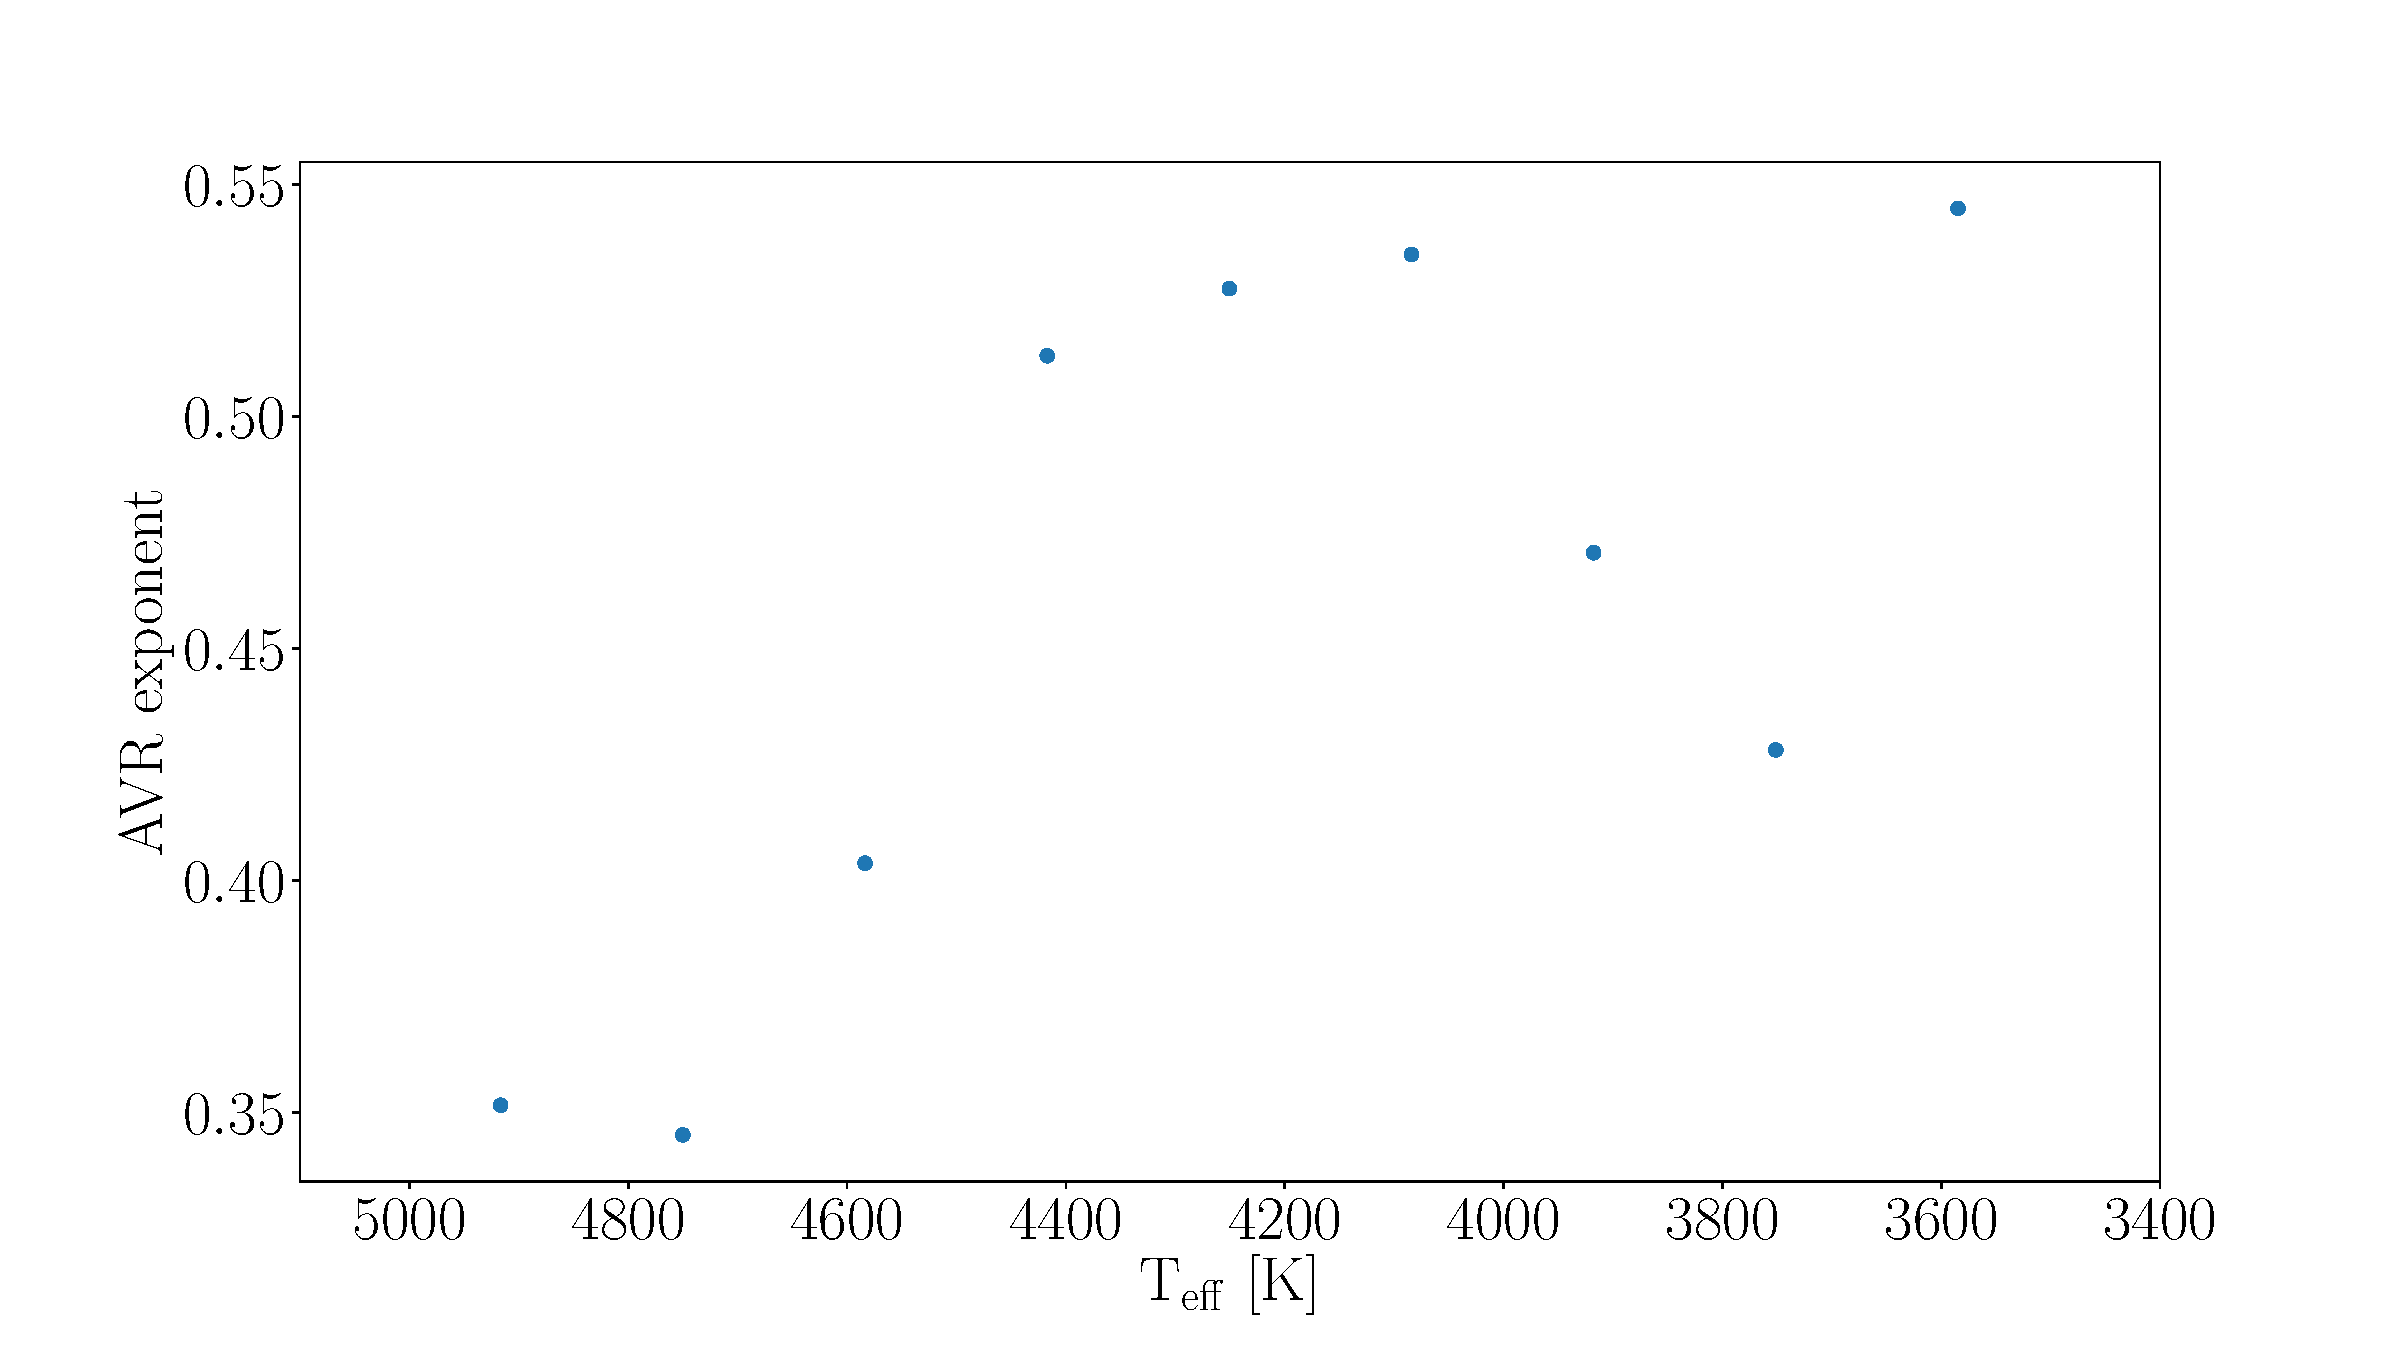
\includegraphics[width=1\textwidth]{AVR_exponent}
% \label{fig:AVR_exponent}
% \end{figure}
% Figure \ref{fig:AVR_exponent} shows the significant rise the in AVR exponent
% as a function of effective temperature.
% The hottest stars in our sample (\teff\ = 4833-5000 K) have a (\vb) AVR
% exponent of 0.39 $\pm$ 0.02 and the coolest (\teff\ = 3500-3667 K) have an
% exponent of 0.74 $\pm$ 0.02.
% The masses of stars in our sample differ by less than a factor of two,
% so mass-dependent heating cannot be entirely responsible for this large spread
% in heating rates.
% \racomment{Need to look into this further.}

% If mass-dependent heating is strongly affecting our data, the exponent of the
% AVR should increase with decreasing effective temperature, \ie\ the heating
% rate should be greater for lower-mass stars.
% Figure \ref{fig:AVR_exponent} shows the AVR exponent does indeed increase with
% decreasing effective temperature, however, the AVR exponent calculated using
% more massive stars from the Geneva Copenhagen Survey (GCS)
% \citep{holmberg2009} is also shown on this plot as a dashed horizontal line.
% Most GCS stars are F and G type: 1-3 times more massive than the K dwarfs used
% in our study.
% If mass-dependent orbital heating is the main cause the rise in velocity
% dispersion with decreasing \teff\ seen in figure \ref{fig:age_cut}, then the
% AVR exponent of the more massive GCS stars should fall {\it below} the AVR
% exponent for the most massive stars in our sample.
% In other words, the dynamical heating rate should be lowest for the highest
% mass stars and highest for the lowest mass stars.
% % nordstrom2004, jorgensen2005,
% These AVR exponents were calculated with different populations of stars,
% subject to different selection effects, so directly comparing them comes with
% some risk.
% The most important difference is that the GCS AVR is calculated using \vz,
% however our AVRs are calculated using \vb\ since most stars in our sample do
% not have radial velocities.
% The median galactic latitude of these \kepler\ stars is 12.3\degrees, with
% latitudes ranging from 5.5\degrees\ to 21.4\degrees, so \vb\ is a relatively
% close approximation to \vz.
% Only 290 out of the 6820 stars in our sample, plotted in color in figure
% \ref{fig:age_cut}, have \gaia\ radial velocities, however we used the ones
% that do to compare the \vz\ AVR to the \vb\ AVR, across all temperatures
% between 3500 and 5000 K.
% For stars with gyrochronal ages between 0.5 and 4.5 Gyr, we measured a \vz\
% AVR exponent of 0.519 $\pm$ ... and a \vb\ AVR exponent of 0.514 $\pm$... .
% The similarity of these two AVR exponents suggests that directly comparing
% these two quantities {\it may} be a reasonable approach.
% For now, given the large difference between the (\vz) AVR exponent of the GCS
% sample and the (\vb) AVR exponent of the hottest stars in our sample, we
% assume that the increased velocity dispersion at cooler temperatures is mostly
% caused by incorrect age-grouping due to an incorrect period-color relation at
% old ages, and that any mass-dependent heating, while it may contribute at a
% low level to this result, is not the dominant driver.
% However, differentiating the effects of mass-dependent heating and the shape
% of the gyrochronology relations is certainly warranted in a follow-up study.
% }

% Figure \ref{fig:age_comparison} shows the ages of star groups, predicted with
% the \citet{angus2019} gyrochronology relation, compared with the ages of star
% groups, predicted with the \citet{holmberg2009} AVR.
% \citet{holmberg2009} only provide an exponent (0.53), not an intercept, for the
% relation between logarithmic age (in Gyr) and logarithmic, \vz\ velocity
% dispersion (in \kms), so we fit the intercept to the mean \vb\ velocity
% dispersion across all temperatures, of our sample.
% \begin{figure}
%   \caption{
%       Ages predicted by the \citet{holmberg2009} \vz\ AVR, against ages
%     predicted by the \citet{angus2019} gyrochronology relation, for stars in
%     different temperature ranges.
% Points are colored by the effective temperature in the center of the \teff\
% bin.
% The dashed line shows the y=x relation.
% Predicted kinematic ages fan out over gyrochronal time, either because the AVR
%     is temperature-dependent or because the gyrochronology relations have an
%     age-dependent period-color relation.
% }
%   \centering
%     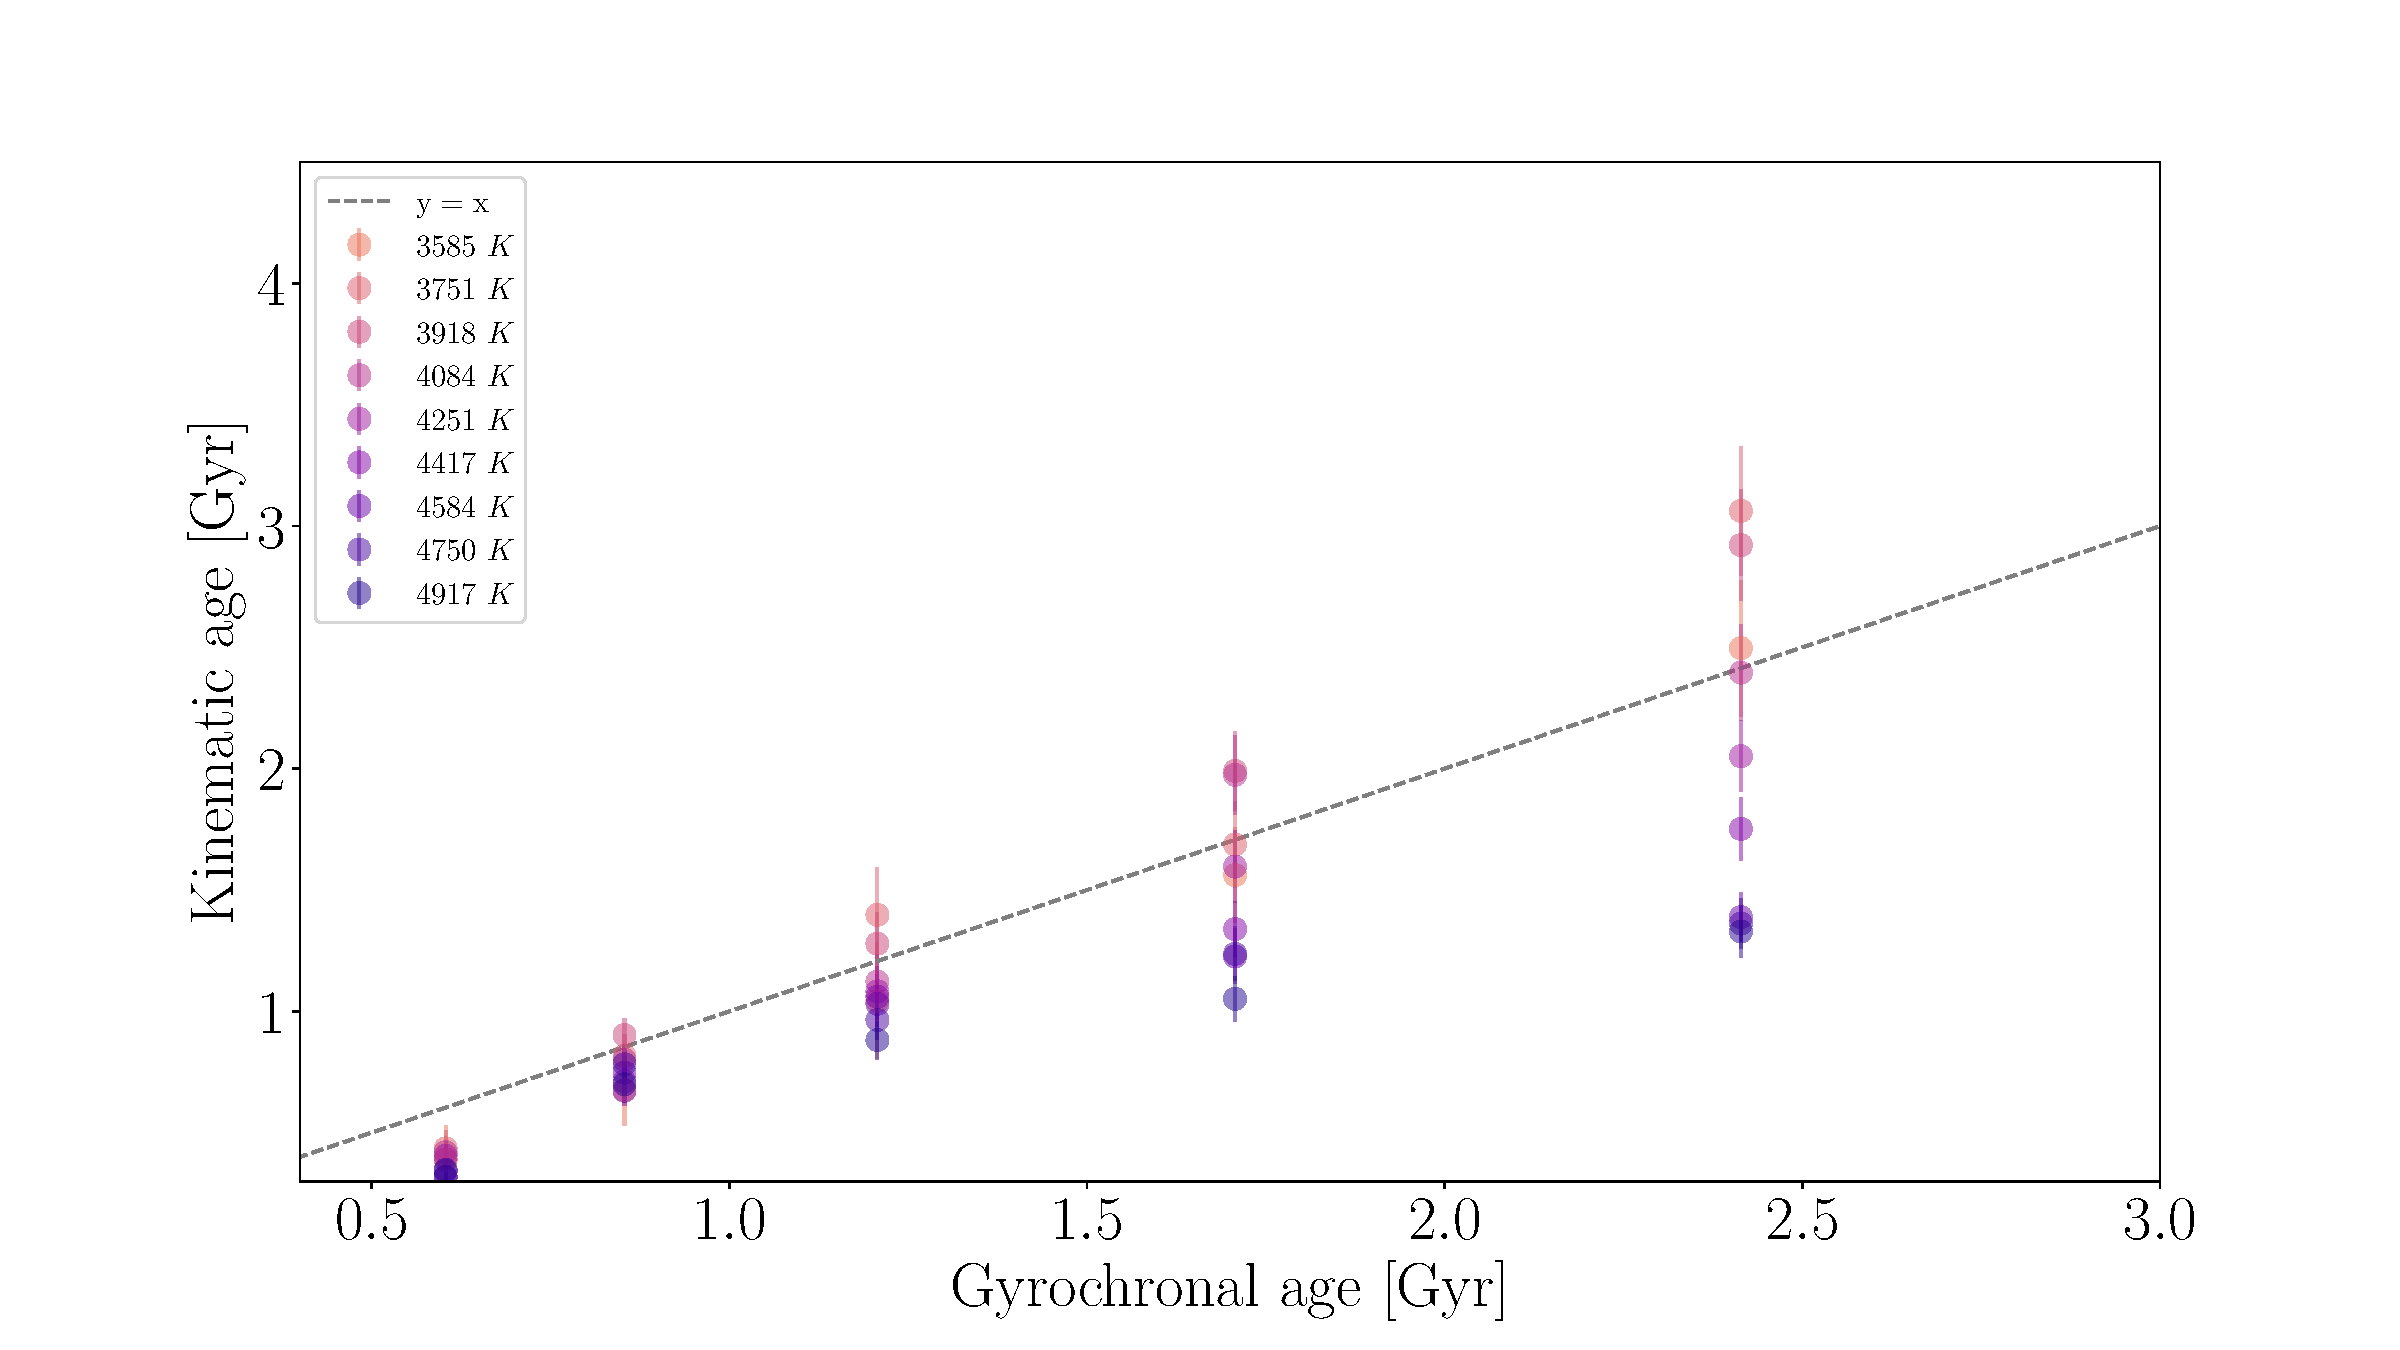
\includegraphics[width=1\textwidth]{age_comparison}
% \label{fig:age_comparison}
% \end{figure}
% Figure \ref{fig:age_comparison} shows a comparison between ages predicted by
% the \citet{holmberg2009} \vz\ AVR (using \vb\ as a proxy for \vz) and ages
% predicted by the \citet{angus2019} gyrochronology relation, for stars in
% different temperature ranges.
% The predicted kinematic ages fan out over gyrochronal time, either because the
% AVR is temperature-dependent or because the gyrochronology relations have an
% age-dependent period-color relation.
% Figure \ref{fig:age_comparion} also suggests that dynamical heating does not
% begin until after around ... Gyr:

% Alternatively, the ages of these young stars could be under-predicted by
% gyrochronology.
% These young stars have similar rotation periods to the Praesepe cluster, which
% was used to calibrate the gyrochronology relation used in this analysis.
% The ages of these young stars should, therefore, be the most accurate of the
% entire sample.
% However, they are tied to the age of the Praesepe cluster, whose age is not
% accurately known.
% \citet{angus2019} adopted an age for Praesepe of 650 Myrs, however the
% kinematic age-prediction for these stars is around 400 Myrs.
% Other studies have assigned a much older age of 800 Myrs to Praesepe
% \citep{brandt2015}.
% If the age assumed for Praesepe in the \citet{angus2019} gyrochronology
% calibration was inaccurate, the entire age {\it scale} would be incorrect.
% However, this is not what figure \ref{fig:age_comparion} shows -- it shows
% that the {\it relative} age of these youngest stars are under-predicted by
% kinematics or over-predicted by gyrochronology.

% If we assume that the rise in velocity dispersions at cooler effective
% temperatures is caused by an inaccurate period-color relation rather than
% mass-dependent dynamical heating, we can estimate what the shape of the
% period-color relations {\it should} be.
% Figure \ref{fig:age_cut} indicates that the period-color relation flattens
% out, so we applied the same analysis to groups of stars with similar rotation
% periods, equivalent to a completely flat period-color relation.
% The top panel of figure \ref{fig:period_cut} shows the \mct\ sample with stars
% in different period ranges plotted in different colors.
% The bottom panel shows the velocity dispersion of each group as a function of
% effective temperature.
% \begin{figure}
%   \caption{
% This figure is similar to figure \ref{fig:age_cut}, with stars divided into
%     period groups rather than age groups.
% The velocity dispersion is more constant across effective temperatures for the
%     most slowly rotating stars, compared to the stars selected with the
%     \citet{angus2019} gyrochronology model, indicating that the gyrochronology
%     models flatten out, and possibly even invert, at old ages.
% }
%   \centering
%     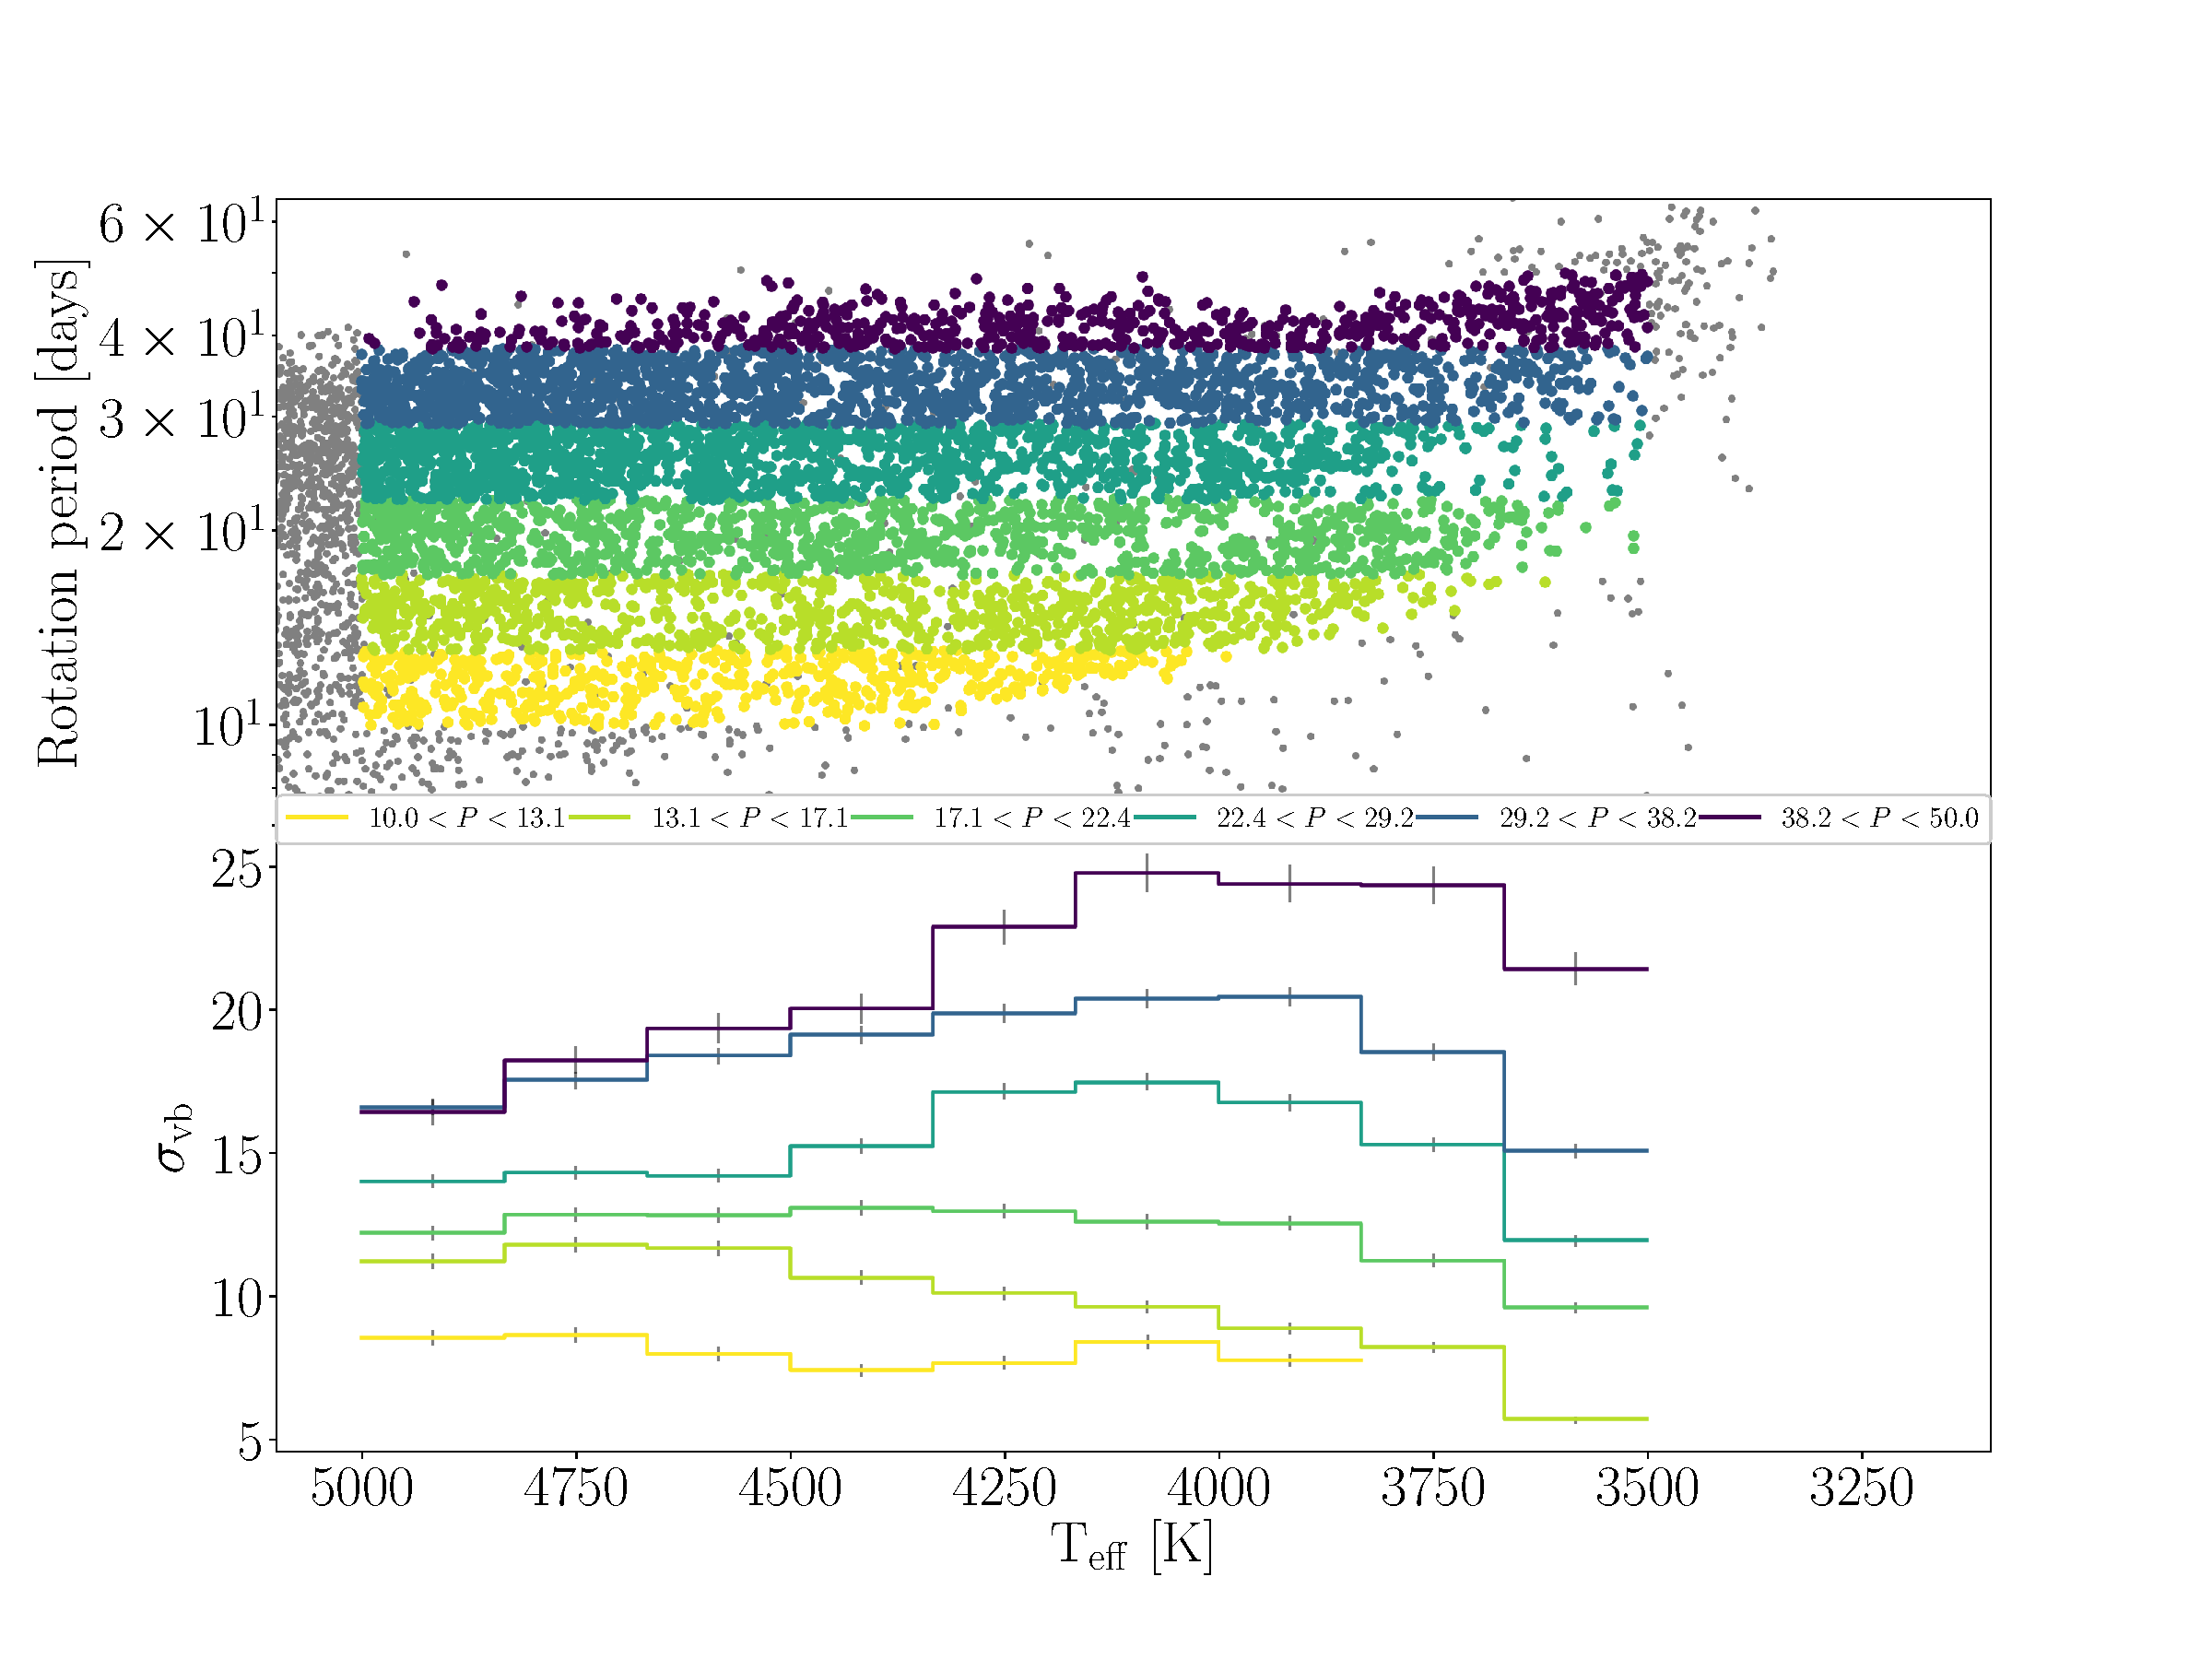
\includegraphics[width=1\textwidth]{period_cut}
% \label{fig:period_cut}
% \end{figure}
% Once again, the velocity dispersion increases with rotation period overall.
% For the most rapidly rotating groups of stars, velocity dispersion decreases
% with \teff\ as expected given the positively sloped period-color relation of
% Praesepe and other young clusters: late K dwarfs rotate more slowly than early
% K dwarfs of the same age.
% Between rotation periods of 15 and 25 days, the temperature dependence of the
% velocity dispersion starts to disappear, indicating that the period-color
% relation becomes flat: late K dwarfs rotate at the same rate as early K dwarfs
% of the same age.
% At long rotation periods, the velocity dispersion still increases with
% effective temperature, although the increase is much more modest compared to
% the oldest stars in figure \ref{fig:age_cut}.

% If we assume the rise in velocity dispersion at cooler effective temperatures
% is caused by an inaccurate period-color relation rather than mass-dependent
% dynamical heating, we can generate a graphical representation of what the
% relations {\it should} look like.

% Aside from the assumption that mass-dependent dynamical heating is {\it not}
% the main cause of the increased velocity dispersion for cooler stars, a number
% of assumptions went into this analysis which should be addressed before a
% strong conclusion about the nature of stellar spin down is drawn.
% There are some potential confounders that could produce trends between
% velocity dispersion and effective temperature, of which the main ones are
% listed below.
% \begin{itemize}

    % \item{{\bf Extinction.}
% Although we dereddened stars before their ages were estimated, if the
    %     reddening values were underestimated, the gyrochronal ages of stars
    %     would be under-estimated.
% This effect would be largest for the late Ks and early Ms, where the shape of
    %     the period-color relation is more steeply sloped, and stars can more
    %     easily move into the wrong age bin with a small perturbation in color
    %     or temperature.
% Old stars would be incorrectly assigned young ages, and this would happen more
    %     often for cooler stars.
% This effect could lead to an increase in velocity dispersion with \teff, even
% if the gyrochronology relation was perfect.}

    % \item{{\bf Mass-dependent orbital heating.}
% A key assumption going into this analysis is that the orbits of all stars are
% heated at the same rate, regardless of their mass.
% However, if the heating mechanism leads to preferential heating of lower mass
% stars, those stars would have a larger velocity dispersion, not caused by
% ageing.
% No strong evidence has yet been provided to show a mass-dependence in orbital
% heating, however this is an extremely difficult exercise because mass and age
% are so strongly correlated.
% The mass-age degeneracy is reduced in the lowest mass stars which represent
    %     the initial mass function of the Solar neighborhood.
% No mass-dependent heating was found by \citet{faherty2009} who looked
% at the velocity dispersions of low-mass stars.
% Another argument against the increased velocity dispersion as a function of
    %     \teff\ being caused by mass-dependent orbital heating, is that heating
    %     acts most strongly at young ages and most weakly at old ages, \ie\ on
    %     a logarithmic timescale.
% This is related to the fact that stars are more difficult to scatter once they
% are on orbits with a large out-of-plane component and they spend more time out
% of the mid-plane.
% Our data show the opposite trend: stars show little mass-dependent heating
    %     before around 1 Gyr.
% Moreover, the stars in the Geneva-Copenhagen study, used to calibrate the AVR
    %     \citep{holmberg2009} are F and G stars, around 1-3 times as massive as
    %     the K stars in our sample.
% % nordstrom2004, jorgensen2005,
% The ages for our sample of K stars, predicted by gyrochronology agree with the
    %     AVR calibrated using F and G stars, which implies that either
    %     mass-dependent heating is a weak effect, or, mass-dependent heating is
    %     strong and, by coincidence, gyrochronology underpredicts the ages of
    %     the early K dwarfs by just the right amount that they still appear to
    %     agree with the \citet{holmberg2009} AVR.
% We therefore expect that the increased velocity dispersion at cooler
    %     temperatures is mostly caused by incorrect age-grouping, \ie\ the
    %     period-color relation is incorrect for old, low-mass stars, and that
    %     any mass-dependent heating, while it may contribute at a low level to
    %     this result, is not the dominant cause.
% }

    % \item{{\bf Selection bias.}
% The \gaia\
% catalog is incompletebecause they are too faint.
% This is simply due to the fact that \kepler's field of view was aimed at low
    %     galactic latitudes, so nearby \kepler\ stars are close to the galactic
    %     plane.
% The heights of stars above the galactic plane, and correspondingly their
    %     velocities and ages, are therefore correlated with distance.
% Almost no high velocity stars appear in our sample at temperatures cooler than
% 3500, which is why the coolest stars were excluded from our sample, however
% the selection function could still affect stars hotter than 3500 K, and is
% suggested by the decrease in velocity dispersions for cool stars of all ages
% in figure \ref{fig:age_cut}.
% However, this selection effect would act in opposition to the observed trend.
% }

% \item{{\bf Weakened magnetic braking.}
% The rotation periods of old stars are faster than predicted by Skumanich-like
% magnetic braking \citep{angus2015, vansaders2016, metcalfe2019}.
% Magnetic braking is expected to become inefficient once stars approach a
% Rossby number (the ratio of rotation period to convective turnover time) of
% around 2 \citep{vansaders2016, vansaders2018}.
% Since hot stars have shallow convection zones and shorter overturn timescales,
% they reach $Ro = 2$ and stop spinning down at shorter rotation periods than
% cool stars.
% For this reason, some of the hotter stars in the sample may already have
% stopped spinning down, and could be much older than a traditional
% gyrochronology relation (like the simple Praesepe-based relation used in this
% analysis) would suggest.
% However, this effect would work to cancel out the trend observed in figure
% \ref{fig:age_cut} because hotter groups of stars would contain more old stars
% with large velocities.
% }

% \item{Stellar or exoplanet companions.}
% Hotter stars are more likely to be binaries.
% This would make synchronized some stars seem younger, more likely for massive
% stars, although really only likely at short rotation periods.

% \end{itemize}

% CONCLUSION

% This indicates that either the \citep{angus2019} period-color relation is
% incorrect, or that mass-dependent dynamical heating is affecting this data set.
% We presented three pieces of evidence that suggest mass-dependent heating
% cannot be responsible for all of the increasing velocity dispersion.

% \begin{itemize}

% \item{
%         No strong evidence for mass-dependent heating has been found among M, L
% and T-type stars.
% These low-mass stars live longer than the current age of the Universe and
%         therefore do not suffer from a mass-age degeneracy
%         \citep{faherty2009}.
% }

% \item{
%         Literature measurements of the (\vz) AVR exponent are slightly higher
% than the value measured from our data set, but calculated using more massive
% stars.
% Mass-dependent dynamical heating should however produce a {\it smaller} AVR
%         exponent for higher-mass stars.
% We acknowledge that the stars in the \mct\ sample, analyzed in this work, are
%         subject to different selection biases than those used to calculate
%         AVRs in the literature \citep{holmberg2009, aumer2009, yu2018}, so
%         drawing direct comparisons between them does not provide a reliable
%         test.
% }

% \item{
%         The differences in the (\vb) AVR exponent between the hottest and
% coolest K dwarfs in our sample are extremely large, spanning values between
% 0.4 and 0.75, yet the difference in mass is less than a factor of two.
% Such a large spread in AVR exponents cannot be explained by mass-dependent
%         heating alone.
% }

% \end{itemize}

% \racomment{Words about the significance of an inverted period-color relation.}

% \racomment{How does the weakened van Saders braking law fit into all this?}

% \racomment{Talk about the fact that the stars in each bin are not necessarily
% the same age.}

% \racomment{Dispersion could be dependent on the selection function.
% We cut stars at high b, because we find that these do lead to a bias.
% We find no evidence for increased velocity dispersion with decreasing teff in
% either vb or vz.
% We find that sigma clipping is necessary for vb but not vz and do not find
% that the outliers are distributed towards higher galactic latitudes.
% }

% \racomment{Trevor suggest that stars forming in clusters could be the reason
% why young stars are so dynamically cool.}

% \racomment{Are there any asteroseismic stars in this sample that could help
% pin down the age?}
